\begin{figure}[h]
\centering
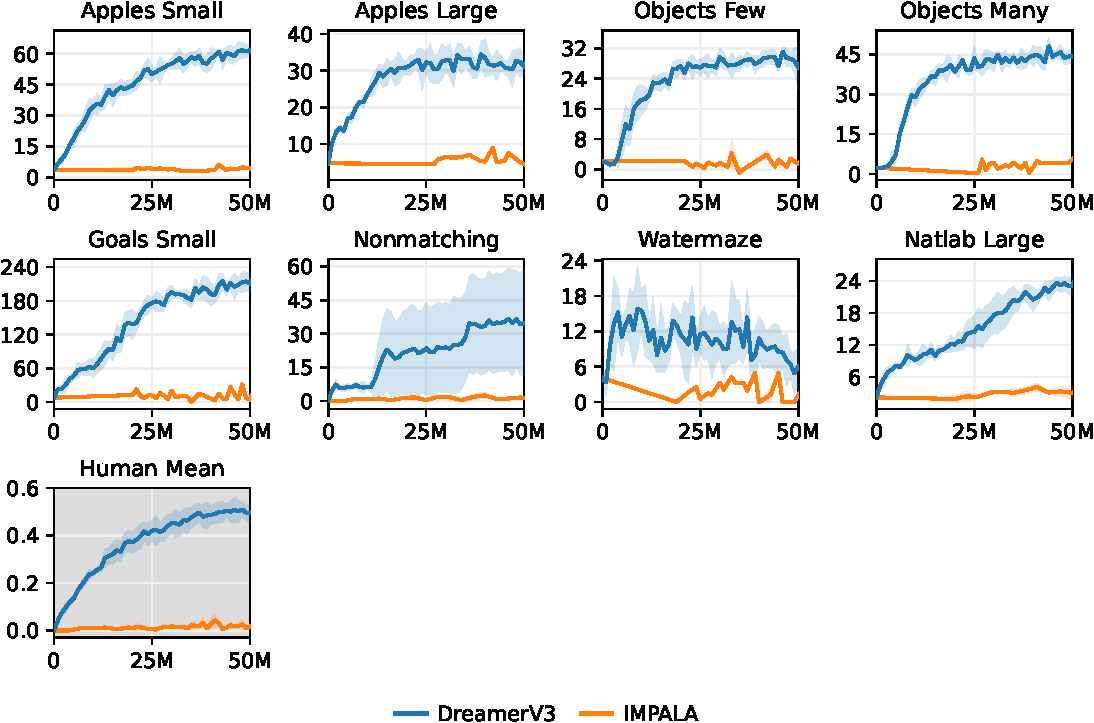
\includegraphics[width=1\linewidth]{dmlab/dmlab}
\caption{DMLab scores with a budget of 50M frames. Separate agents were trained for each task, corresponding to the IMPALA Experts method in \citet{espeholt2018impala}. Data efficiency is not the goal of IMPALA and it might be possible to tune it for improved data efficiency. Longer training curves and asymptotic performance of IMPALA are included in \cref{sec:dmlab_eff}.}
\label{fig:dmlab}
\end{figure}

\section*{Introduction}
\label{sec:intro}

% Reinforcement learning has enabled computers to solve individual tasks by interaction with an environment, such as surpassing humans in the games of Go and Dota \citep{silver2016alphago,openai2018dota}.
% However, applying algorithms to new application domains, for example from board games to video games or robotics tasks, typically requires expert knowledge and computational resources for tuning the algorithm \citep{andrychowicz2020whatmatters}.
% Moreover, this brittleness and the reliance on specific neural architectures hinders scaling to complex domains that require larger models \citep{parisotto2020stabilizing,sinha2020d2rl}.
% Different domains pose unique challenges, including action spaces, input ranges and shapes, and rewards frequencies and scales---all of which can stagnate learning.
% Developing a general algorithm that learns to solve new domains without tuning would remove this barrier and open reinforcement learning up to a wide range of practical applications.

% Reinforcement learning has enabled computers to solve individual tasks through interaction, such as surpassing humans in the games of Go and Dota \citep{silver2016alphago,openai2018dota}.
% However, applying algorithms to new application domains, for example from board games to video games or robotics tasks, requires expert knowledge and computational resources for tuning the algorithms or developing new ones \citep{andrychowicz2020whatmatters}.
% This brittleness also hinders scaling to complex domains that require large models, which are expensive to tune.
% Different domains pose unique challenges, motivating the development of specialized algorithms, such as for continuous control \citep{lillicrap2015ddpg,gu2016naf}, sparse rewards \citep{jaderberg2016unreal,riedmiller2018sparseplay}, image inputs \citep{anand2019ataristaterep,laskin2020rad}, and 3D worlds \citep{mirchev2020argmax3d,driess2022nerfrl}.
% Creating a general algorithm that learns to solve new domains out of the box would remove the need for expert knowledge and open up reinforcement learning to a wide range of practical applications.

Reinforcement learning has enabled computers to solve individual tasks through interaction, such as surpassing humans in the games of Go and Dota \citep{silver2016alphago,openai2018dota}.
However, applying algorithms to new application domains, for example from board games to video games or robotics tasks, requires expert knowledge and computational resources for tuning the algorithms \citep{andrychowicz2020whatmatters}.
This brittleness also hinders scaling to large models that are expensive to tune.
Different domains pose unique learning challenges that have prompted specialized algorithms, such as for continuous control \citep{lillicrap2015ddpg,gu2016naf}, sparse rewards \citep{jaderberg2016unreal,riedmiller2018sparseplay}, image inputs \citep{anand2019ataristaterep,laskin2020rad}, and spatial environments \citep{mirchev2020argmax3d,driess2022nerfrl}.
Creating a general algorithm that learns to master new domains out of the box---without tuning---would overcome the barrier of expert knowledge and open up reinforcement learning to a wide range of practical applications.

We present DreamerV3, a general and scalable algorithm that masters a wide range of domains with fixed hyperparameters, outperforming specialized algorithms.
DreamerV3 learns a world model \citep{sutton1991dyna,ha2018worldmodels,hafner2018planet} from experience for rich perception and imagination training.
The algorithm consists of 3 neural networks: the world model predicts future outcomes of potential actions, the critic judges the value of each situation, and the actor learns to reach valuable situations.
We enable learning across domains with fixed hyperparameters by transforming signal magnitudes and through robust normalization techniques.
To provide practical guidelines for solving new challenges, we investigating the scaling behavior of DreamerV3.
Notably, we demonstrate that increasing the model size of DreamerV3 monotonically improves both its final performance and data-efficiency.

The popular video game Minecraft has become a focal point of reinforcement learning research in recent years, with international competitions held for learning to collect diamonds in Minecraft \citep{guss2019minerl}.
Solving this challenge without human data has been widely recognized as a milestone for artificial intelligence because of the sparse rewards, exploration difficulty, and long time horizons in this procedurally generated open-world environment.
Due to these obstacles, previous approaches resorted to human expert data and manually-crafted curricula \citep{baker2022vpt,kanitscheider2021minecraftcurriculum}.
DreamerV3 is the first algorithm to collect diamonds in Minecraft from scratch, solving this challenge.

We summarize the four key contributions of this paper as follows:
\begin{itemize}[topsep=-.5ex]
\setlength{\itemsep}{.2ex}
\setlength{\parskip}{0pt}
\item We present DreamerV3, a general algorithm that learns to master diverse domains while using fixed hyperparameters, making reinforcement learning readily applicable.
\item We demonstrate the favorable scaling properties of DreamerV3, where increased model size leads to monotonic improvements in final performance and data-efficiency.
\item We perform an extensive evaluation, showing that DreamerV3 outperforms more specialized algorithms across domains, and release the training curves of all methods to facilitate comparison.
\item We find that DreamerV3 is the first algorithm to collect diamonds in Minecraft from scratch without human data or curricula, solving a long-standing challenge in artificial intelligence.
% \item On DMLab tasks, DreamerV3 reaches and exceeds the final performance of the scalable IMPALA algorithm while using 130 times fewer interactions.
\end{itemize}
